\documentclass[tikz,border=10pt]{standalone}
\usetikzlibrary{calc}

\begin{document}
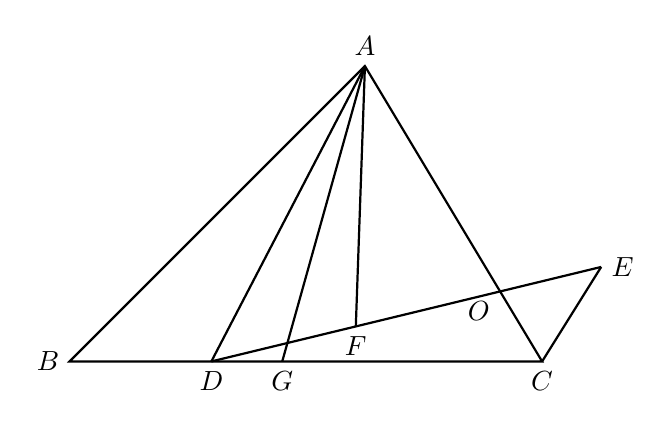
\begin{tikzpicture}[scale=1.5, thick,
    dot/.style={circle, fill=black, inner sep=1pt}]

    % 1. 定义核心顶点坐标 (手动拟合图像比例)
    \coordinate (B) at (0,0);
    \coordinate (C) at (4,0);
    \coordinate (A) at (2.5,2.5);
    \coordinate (D) at (1.2,0);
    \coordinate (G) at (1.8,0);
    \coordinate (E) at (4.5,0.8);
    
    % 计算交点 O (AC 与 DE 的交点)
    \coordinate (O) at (intersection of A--C and D--E);
    % 设定 F 点在线段 DE 上 (根据视觉大致位置定于 DE 中间偏左)
    \coordinate (F) at ($(D)!0.5!(O)$);

    % 2. 绘制所有线段
    \draw (B) -- (C) -- (A) -- cycle; % 主三角形 ABC
    \draw (D) -- (E);             % 线段 DE
    \draw (A) -- (D);             % 连线 AD
    \draw (A) -- (G);             % 连线 AG
    \draw (A) -- (F);             % 连线 AF
    \draw (C) -- (E);             % 连线 CE
    
    % 3. 标注顶点标签
    \node[anchor=east] at (B) {$B$};
    \node[anchor=north] at (D) {$D$};
    \node[anchor=north] at (G) {$G$};
    \node[anchor=north] at (C) {$C$};
    \node[anchor=south] at (A) {$A$};
    \node[anchor=west] at (E) {$E$};
    \node[anchor=north] at (F) {$F$};
    \node[anchor=north east] (O_node) at (O) {$O$};

\end{tikzpicture}
\end{document}